\documentclass[a4paper,12pt]{article}
\usepackage{tikz}
\usepackage{geometry}
\usepackage{amsmath}
\usepackage{parskip}
\geometry{margin=1in}

\begin{document}

\begin{center}
  \LARGE Free-body diagrams: two boxes on a smooth incline and a hanging sack\\[6pt]
  \large Incline angle $15^\circ$, boxes of mass $20\ \mathrm{kg}$ and $25\ \mathrm{kg}$, hanging sack mass $M$
\end{center}

\vspace{8pt}

%---------------- Overall setup ----------------
\begin{center}
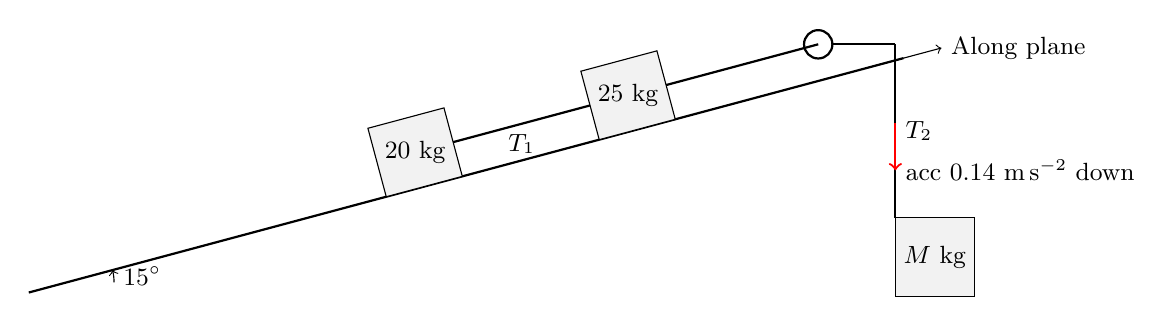
\begin{tikzpicture}[scale=1.0, every node/.style={font=\small}]
  \def\ang{15}
  % Draw incline (rotate a horizontal line)
  \begin{scope}[rotate=\ang]
    \draw[thick] (-0.5,0) -- (11,0);
    % ground reference
    \draw[->] (10.5,0) -- (11.5,0) node[right]{Along plane};
  \end{scope}

  % Place boxes on rotated coordinates
  \begin{scope}[rotate=\ang]
    % 25 kg box (up the slope)
    \draw[fill=gray!10] (7.0,0) rectangle (8.0,0.9) node[midway] {25 kg};
    % 20 kg box (down the slope, behind)
    \draw[fill=gray!10] (4.2,0) rectangle (5.2,0.9) node[midway] {20 kg};
    % rope between boxes (parallel to plane)
    \draw[thick] (5.2,0.45) -- (7.0,0.45) node[midway,below] {$T_1$};
    % cable from 25 kg box to pulley
    \draw[thick] (8.0,0.45) -- (10.0,0.45);
    % pulley (drawn in original orientation)
  \end{scope}

  % Pulley in unrotated orientation (position transform)
  % Compute pulley centre by rotating point (10,0.45) by ang about origin:
  \coordinate (pulley) at ({10*cos(\ang) - 0.45*sin(\ang)}, {10*sin(\ang) + 0.45*cos(\ang)});
  \draw[thick] (pulley) circle (0.18);
  % small tangent point to indicate cable over pulley
  \draw[thick] (pulley) ++(0:0.18) -- ++(0.8,0) node[right] {};
  % hanging rope and sack
  \draw[thick] (pulley) ++(0:0.18) -- ++(0.8,0) coordinate (ropeend);
  \draw[thick] (ropeend) -- ++(0,-2.2) node[midway,right] {$T_2$};
  % sack
  \draw[fill=gray!10] (ropeend) ++(0,-2.2) rectangle ++(1,-1.0) node[midway] {$M$ kg};
  % label acceleration of sack
  \draw[->,red,thick] (ropeend) ++(0,-1.0) -- ++(0,-0.6) node[right,black] {acc $0.14\ \mathrm{m\,s^{-2}}$ down};

  % Indicate angle at origin
  \draw[->] (0.6,0) arc (0:\ang:0.6) node[midway,right] {$15^\circ$};
\end{tikzpicture}
\end{center}

\vspace{12pt}

%---------------- FBDs ----------------
\begin{center}
  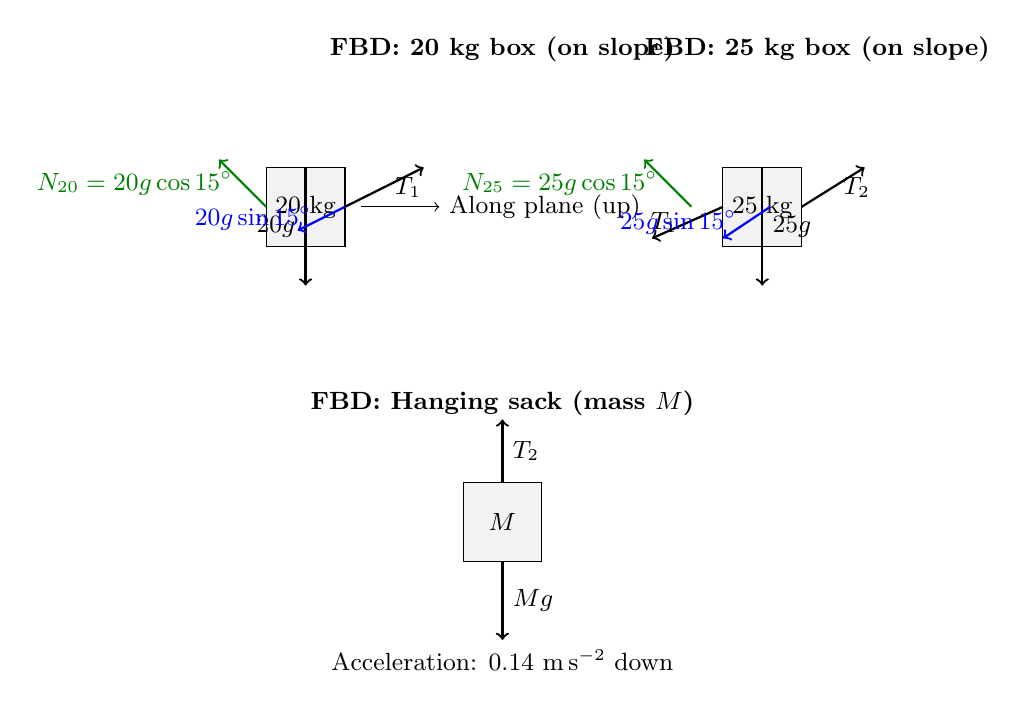
\begin{tikzpicture}[scale=1.0, every node/.style={font=\small}]
    % 20 kg box FBD
    \node at (0,0.5) {\textbf{FBD: 20 kg box (on slope)}};
    % Draw box
    \draw[fill=gray!10] (-3,-2) rectangle (-2,-1) node[midway] {20 kg};
    % Draw slope direction arrow for reference
    \draw[->] (-1.8,-1.5) -- (-0.8,-1.5) node[right] {Along plane (up)};
    % Forces: T1 up the plane (parallel)
    \draw[->,thick] (-2.0,-1.5) -- (-1.0,-1.0) node[midway,above,right] {$T_1$};
    % Weight vertical down
    \draw[->,thick] (-2.5,-1) -- (-2.5,-2.5) node[midway,left] {$20g$};
    % Component of weight parallel to plane (down the slope)
    \draw[->,thick,blue] (-2.0,-1.5) -- (-2.6,-1.8) node[midway,below,left] {$20g\sin 15^\circ$};
    % Normal reaction perpendicular to plane
    \draw[->,thick,green!50!black] (-3.0,-1.5) -- (-3.6,-0.9) node[midway,left] {$N_{20}=20g\cos 15^\circ$};

    % 25 kg box FBD
    \node at (4,0.5) {\textbf{FBD: 25 kg box (on slope)}};
    \draw[fill=gray!10] (2.8,-2) rectangle (3.8,-1) node[midway] {25 kg};
    % T2 up the plane
    \draw[->,thick] (3.8,-1.5) -- (4.6,-1.0) node[midway,above,right] {$T_2$};
    % T1 pulling down the plane (from 20kg)
    \draw[->,thick] (2.8,-1.5) -- (1.9,-1.9) node[midway,below,left] {$T_1$};
    % Weight vertical down
    \draw[->,thick] (3.3,-1) -- (3.3,-2.5) node[midway,right] {$25g$};
    % Component of weight parallel to plane (down)
    \draw[->,thick,blue] (3.4,-1.5) -- (2.8,-1.9) node[midway,below,left] {$25g\sin 15^\circ$};
    % Normal reaction
    \draw[->,thick,green!50!black] (2.4,-1.5) -- (1.8,-0.9) node[midway,left] {$N_{25}=25g\cos 15^\circ$};

    % Hanging sack FBD
    \node at (0,-4.0) {\textbf{FBD: Hanging sack (mass $M$)}};
    \draw[fill=gray!10] (-0.5,-6) rectangle (0.5,-5) node[midway] {$M$};
    % Tension up
    \draw[->,thick] (0,-5) -- (0,-4.2) node[midway,right] {$T_2$};
    % Weight down
    \draw[->,thick] (0,-6) -- (0,-7) node[midway,right] {$Mg$};
    % Acceleration label
    \node[below] at (0,-7) {Acceleration: $0.14\ \mathrm{m\,s^{-2}}$ down};
  \end{tikzpicture}
\end{center}

\vspace{8pt}

\noindent Notes (useful while solving):
\begin{itemize}
  \item For the boxes, resolve forces parallel to the plane: \\
    20 kg box: $T_1 - 20g\sin 15^\circ = 20 a$ (along plane).\\
    25 kg box: $T_2 - T_1 - 25g\sin 15^\circ = 25 a$.
  \item For the hanging sack: $Mg - T_2 = M \times 0.14$ (downwards).
  \item Normal reactions: $N_{20}=20g\cos 15^\circ$, $N_{25}=25g\cos 15^\circ$.
\end{itemize}

\end{document}